\DiaryEntry{Klein-4 Group}{2016-10-24}{Algebra}

\subsection{Definition}\label{definition}

The Klein-4 Group \(\mathbb{K}_4\) is defined by the following equations

\[
a^2 = b^2 = (ab)^2 = e
\]

and typically \(ab\) will be denoted as \(ab = c\). In order to write
down the Cayley table, three products are missing: \(ab, ac\) and
\(bc\).

\[
\begin{array}{c|cccc}
\star   & e     & a    & b   & c     \\
\hline
e       & e     & a    & b   & c     \\
a       & a     & e    & ?   & ?     \\
b       & b     & ?    & e   & ?     \\
c       & c     & ?    & ?   & e
\end{array}
\]

For the product \(ab\) we have two options: (i) \(ab = b\), (ii)
\(ab = c\). Option (i) does not work, as it would imply that \(a = e\)
and we already have one identity element. Therefore, \(ab = c\),
\(ac = b\) and we arrive at

\[
\begin{array}{c|cccc}
\star   & e     & a    & b   & c     \\
\hline
e       & e     & a    & b   & c     \\
a       & a     & e    & c   & b     \\
b       & b     & c    & e   & ?     \\
c       & c     & b    & ?   & e
\end{array}
\]

There is only one question mark left and the remaining identites allow
to uniquely deduce \(bc = a\). We therefore have

\[
\begin{array}{c|cccc}
\star   & e     & a    & b   & c     \\
\hline
e       & e     & a    & b   & c     \\
a       & a     & e    & c   & b     \\
b       & b     & c    & e   & a     \\
c       & c     & b    & a   & e
\end{array}
\]

\subsection{Characteristics}\label{characteristics}

\begin{itemize}
\item
  All non-identity elements have order two; i.e.
  \(x \in \mathbb{K}_4 \rightarrow x^2 = e\). In other words, the main
  diagonal of the Cayley table contains only the identity element \(e\).
\item
  The group is isomorphic to \(\mathbb{Z}_2 \oplus \mathbb{Z}_2\) and
  can be represented as the pairs \(\{(0,0), (0,1), (1,0), (1,1)\}\)
  under component-wise addition modulo-2 (\(\{0,0\}\) being the identity
  element) or as bit string \(\{00, 01, 10, 11\}\) under component-wise
  xor-operation (\(\{00\}\) being the identity element).
\item
  Another isomorphism is given by the mapping
  \(e \rightarrow 1, a \rightarrow 3, b \rightarrow 5, c \rightarrow 7\)
  under multiplication modulo-8
  (\(a b \rightarrow 3 \times 5 = 15 = 7 \mod 8\)).
\item
  The Klein-4 group is an elementary abelian group as every nontrivial
  element has prime order \(p = 2\). This is also called a Boolean
  group.
\end{itemize}

\subsection{Symmetric Difference}\label{symmetric-difference}

The symmetric difference \(A \triangle B\) of two sets A and B is the
set of elements which are in either of the sets but not in their
intersection; i.e.~it is the union of the two sets, minus their
intersection.

The Figure below illustrates the concept.

\begin{figure}
\centering
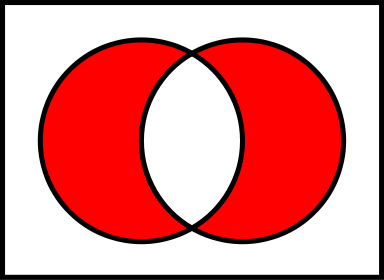
\includegraphics{images/symmetric_difference.png}
\caption{Page1}
\end{figure}

As an example, consider \(A = \{1,2,3\}\) and \(B = \{3,4\}\). Then
\(A \triangle B = \{1,2,4\}\) (it does not contain \(3\) as this element
is contained in both \(A\) and \(B\) and therefore in the intersection).

By its very definition, the symmetric difference is symmetric; i.e.
\(A \triangle B = B \triangle A\). Other cases of interest are:

\begin{itemize}
\item
  The symmetric difference of the empty set and any set is the set:
  \(\{\} \triangle A = A\).
\item
  The symmetric difference of a set with itself is the empty set
  \(A \triangle A = \{\}\).
\item
  The symmetric difference of two disjoint sets is equal their union:
  \(A \cap B = \{\} \rightarrow A \triangle B = A \cup B\).
\end{itemize}

\subsubsection{Connection to Klein-4
Group}\label{connection-to-klein-4-group}

The Klein-4 group is the group generated by the symmetric difference
\(\triangle\) as the binary operation on the subsets of a powerset of a
set with two elements. We have the following power set
\(\{\}, \{\alpha\}, \{\beta\}, \{\alpha, \beta\}\).

The empty set is the identity element of the group
(\(A \triangle \{\} = A\)) and the Cayley table looks as follows:

\[
\begin{array}{c|cccc}
\star   & \{\}     & \{\alpha \}    & \{\beta\}   & \{\alpha, \beta\}     \\
\hline
\{\}       & \{\}     & \{\alpha\}    & \{\beta\}   & \{\alpha, \beta\}     \\
\{\alpha\}       & \{\alpha\}     & \{\}    & \{\alpha, \beta\}   & \{\beta\}     \\
\{\beta\} & \{\beta\}     & \{\alpha, \beta\}    & \{\}   & \{\alpha\}     \\
\{\alpha, \beta\}       & \{\alpha, \beta\}     & \{\beta\}    & \{\alpha\}   & \{\}
\end{array}
\]

\subsubsection{Generalization}\label{generalization}

If we consider powersets of sets with more than two elements, we can -
in a way - generalize the Klein-4 Group. The Klein-4 group has the
property that \(a^2 = b^2 = c^2 = e\) and with the reasoning from above,
\(A \triangle A = \{\}\). Therefore, this property of the Klein-4 group
is kept.

The next group is based on the power set of a set with 3 elements $\alpha \beta, \gamma:$\\ $\{\}, \{\alpha\}, \{\beta\}, \{\gamma\}, \{\alpha, \beta\}, \{\alpha, \gamma\}, \{\beta, \gamma\}, \{\alpha, \beta, \gamma\}$.
